
\documentclass[border=8pt, multi, tikz]{standalone} 
\usepackage{import}
\subimport{./layers/}{init}
\usetikzlibrary{positioning}
\usetikzlibrary{calc}
\usetikzlibrary{3d} %for including external image 

\def\ConvColor{rgb:yellow,5;red,2.5;white,5}
\def\ConvReluColor{rgb:yellow,5;red,5;white,5}
\def\PoolColor{rgb:red,1;black,0.3}
\def\UnpoolColor{rgb:blue,2;green,1;black,0.3}
\def\FcColor{rgb:blue,5;red,2.5;white,5}
\def\FcReluColor{rgb:blue,5;red,5;white,4}
\def\SoftmaxColor{rgb:magenta,5;black,7}   
\def\SumColor{rgb:blue,5;green,15}
\def\TensorIoColor{rgb:black,3.5;white,14}

\newcommand{\copymidarrow}{\tikz \draw[-Stealth,line width=0.8mm,draw={rgb:blue,4;red,1;green,1;black,3}] (-0.3,0) -- ++(0.3,0);}

\begin{document}
\begin{tikzpicture}
\tikzstyle{connection}=[ultra thick,every node/.style={sloped,allow upside down},draw=\edgecolor,opacity=0.7]
\tikzstyle{copyconnection}=[ultra thick,every node/.style={sloped,allow upside down},draw={rgb:blue,4;red,1;green,1;black,3},opacity=0.7]
\tikzset{connection path xz mid/.style={
  ultra thick,
  draw=\edgecolor,
  opacity=0.7,
  decoration={
    markings,
    mark=at position 0.5 with {\arrow[scale=1.12]{Stealth[length=4.5mm,width=3.4mm,line width=0.8mm,fill={\edgecolor}]}}
  },
  postaction={decorate}
}}
\tikzset{connection path xy mid/.style={
  ultra thick,
  draw=\edgecolor,
  opacity=0.7,
  decoration={
    markings,
    mark=at position 0.5 with {\arrow[scale=1.12]{Stealth[length=4.5mm,width=3.4mm,line width=0.8mm,fill={\edgecolor}]}}
  },
  postaction={decorate}
}}
\tikzset{connection path plain/.style={
  ultra thick,
  draw=\edgecolor,
  opacity=0.7
}}

\node[canvas is zy plane at x=0, transform shape, inner sep=0pt] (inputstrip0) at (-3,0,0) {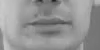
\includegraphics[width=9.000cm,height=4.400cm]{input_bundle/000.png}};

\node[canvas is zy plane at x=0, transform shape, inner sep=0pt] (inputstrip1) at (-2.25,0,0) {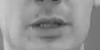
\includegraphics[width=9.000cm,height=4.400cm]{input_bundle/001.png}};

\node[canvas is zy plane at x=0, transform shape, inner sep=0pt] (inputstrip2) at (-1.5,0,0) {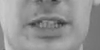
\includegraphics[width=9.000cm,height=4.400cm]{input_bundle/002.png}};

\node[canvas is zy plane at x=0, transform shape, inner sep=0pt] (inputstrip3) at (-0.75,0,0) {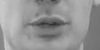
\includegraphics[width=9.000cm,height=4.400cm]{input_bundle/003.png}};

\pic[shift={(0,0,0)}] at (0,0,0)
    {Box={
        name=input,
        caption={\parbox{1.9cm}{\raggedright \mbox{Input}\\$C:1$}},
        xlabel={{ 1, }},
        zlabel=\mbox{$50\times100$},
        fill=\ConvColor,
        height=22,
        width=1.5,
        depth=45
        }
    };

\pic[shift={ (2.0,0,0) }] at (input-east) 
    {RightBandedBox={
        name=rb1,
        caption={\parbox{2.5cm}{\raggedright ResBlock3D\\$C:1\to128$}},
        xlabel={{ 128, 128 }},
        zlabel={\mbox{$25\times50$}},
        fill=\ConvColor,
        bandfill=\ConvReluColor,
        height=17,
        width={ 4 , 4 },
        depth=35
        }
    };

\draw [connection]  (input-east)    -- node {\midarrow} (rb1-west);

\pic[shift={ (2.0,0,0) }] at (rb1-east) 
    {RightBandedBox={
        name=rb2,
        caption={\parbox{2.5cm}{\raggedright ResBlock3D\\$C:128\to256$}},
        xlabel={{ 256, 256 }},
        zlabel={\mbox{$13\times25$}},
        fill=\ConvColor,
        bandfill=\ConvReluColor,
        height=13,
        width={ 8 , 8 },
        depth=25
        }
    };

\draw [connection]  (rb1-east)    -- node {\midarrow} (rb2-west);

\pic[shift={ (2.0,0,0) }] at (rb2-east) 
    {RightBandedBox={
        name=rb3,
        caption={\parbox{2.5cm}{\raggedright ResBlock3D\\$C:256\to512$}},
        xlabel={{ 512, 512 }},
        zlabel={\mbox{$7\times13$}},
        fill=\ConvColor,
        bandfill=\ConvReluColor,
        height=8,
        width={ 16 , 16 },
        depth=15
        }
    };

\draw [connection]  (rb2-east)    -- node {\midarrow} (rb3-west);

\pic[shift={ (2.0,0,0) }] at (rb3-east) 
    {Box={
        name=pool,
        caption={\parbox{1.2cm}{\raggedright AAP}},
        zlabel=\mbox{$4\times4$},
        xlabel={{512, }},
        fill=\PoolColor,
        opacity=0.5,
        height=4,
        width=16,
        depth=4
        }
    };

\draw [connection]  (rb3-east)    -- node {\midarrow} (pool-west);

\pic[shift={(2.0,0,0)}] at (pool-east)
    {Box={
        name=flatten,
        caption={\parbox{2.4cm}{\raggedright \mbox{Flatten}\\\mbox{$C\times4\times4\to8192$}}},
        xlabel={{ 1, }},
        zlabel=$8192$,
        fill=\ConvColor,
        height=1.5,
        width=1.5,
        depth=64
        }
    };

\draw [connection]  (pool-east)    -- node {\midarrow} (flatten-west);

\draw[densely dashed]
    (pool-nearnortheast) -- (flatten-nearnorthwest)
    (pool-nearsoutheast) -- (flatten-nearsouthwest)
    (pool-farsoutheast) -- (flatten-farsouthwest)
    (pool-farnortheast) -- (flatten-farnorthwest)
;

\pic[shift={ (2.0,0,0) }] at (flatten-east) 
    {RightBandedBox={
        name=proj,
        caption={\parbox{2.6cm}{\raggedright Linear+ReLU\\\mbox{$8192\to D:512$}}},
        xlabel={{ 1, }},
        zlabel={$512$},
        fill=\ConvColor,
        bandfill=\ConvReluColor,
        height=1.5,
        width={ 1.5 },
        depth=19
        }
    };

\draw [connection]  (flatten-east)    -- node {\midarrow} (proj-west);

\pic[shift={ (1.5,0,0) }] at (proj-east) 
    {RightBandedBox={
        name=tcn1,
        caption={\parbox{2.5cm}{\raggedright \mbox{TCN (3 blocks)}\\\mbox{$D:512\to 512$}}},
        xlabel={{"$T$", }},
        zlabel={$512$},
        fill=\ConvColor,
        bandfill=\ConvReluColor,
        height=1.5,
        width={ 28 },
        depth=19
        }
    };

\draw [connection]  (proj-east)    -- node {\midarrow} (tcn1-west);

\pic[shift={ (1.0,0,0) }] at (tcn1-east) 
    {RightBandedBox={
        name=tcn2,
        caption={\parbox{2.5cm}{\raggedright \mbox{TCN (3 blocks)}\\\mbox{$D:512\to 512$}}},
        xlabel={{"$T$", }},
        zlabel={$512$},
        fill=\ConvColor,
        bandfill=\ConvReluColor,
        height=1.5,
        width={ 28 },
        depth=19
        }
    };

\draw [connection]  (tcn1-east)    -- node {\midarrow} (tcn2-west);

\pic[shift={(1.8,0,0)}] at (tcn2-east)
    {Box={
        name=fc,
        caption={\parbox{2.2cm}{\raggedright FC\\\mbox{$D:512\to |\mathcal{V}|:28$}}},
        xlabel={{ 1, }},
        zlabel=$512$,
        fill=\FcColor,
        height=1.5,
        width=1.5,
        depth=19
        }
    };

\draw [connection]  (tcn2-east)    -- node {\midarrow} (fc-west);

\pic[shift={(2.0,0,0)}] at (fc-east) 
    {Box={
        name=out,
        caption={\parbox{1.9cm}{\raggedright logits\\$|\mathcal{V}|:28$}},
        xlabel={{" ","dummy"}},
        zlabel=\mbox{$\vert\mathcal{V}\vert{=}28$},
        fill=\SoftmaxColor,
        opacity=0.8,
        height=1.5,
        width=1.5,
        depth=10
        }
    };

\draw [connection]  (fc-east)    -- node {\midarrow} (out-west);

\end{tikzpicture}
\end{document}
